\documentclass[twocolumn, 11pt]{article}
\usepackage[margin=0.5in]{geometry}
\usepackage{booktabs}
\usepackage{multirow}
\usepackage{graphicx}
\usepackage{paralist}
\usepackage{subcaption}

\setlength{\columnsep}{0.3in}

\title{CS224S Assignment 3}
\author{Milind Ganjoo\\\texttt{mganjoo@cs.stanford.edu}
\and%
Stephanie Lynne Pancoast\\\texttt{pancoast@stanford.edu}
\and%
Sebastian Schuster\\\texttt{sebschu@stanford.edu}}
\date{}

\begin{document}

\maketitle
\pagenumbering{gobble}
\section{Improving the monophone acoustic model}\label{sec:improved-mono}

Initially, we tried various values for the five parameters to determine the
optimal values for the male-only training set using \emph{Mel-frequency cepstral
coefficients (MFCCs)}, with no normalization or triphone features. In this
section we describe our method for tuning the parameters, present the results,
and include a discussion as to why certain parameter adjustments showed improved
test results with respect to the baseline system.

\subsection{Parameters}

\paragraph{Number of iterations (\texttt{num\_iters})} We tried 10, 20 and 30 iterations and found 20
iterations to show the lowest word and sentence error rate. 10 iterations was
not sufficient for the Gaussian HMM model to converge, whereas after 30
iterations the improvement seen at 20 has plateaued and begun to worsen.

\paragraph{Silence boost factor (\texttt{boost\_silence})} The default value for
this parameter was 1, indicating no special treatment being given to the
likelihoods of GMMs corresponding to the silence phones. By increasing this
parameter, we are indicating it is more likely for a silence phone to occur, and
a decrease in the parameter makes the model less likely to choose a silence
phone. We tried values between 0.3 and 1.5, and found the best performance
results by setting \texttt{boost\_silence} to 0.5. This is equivalent to halving
the weights for all models that correspond to the silence decreased.

The silence class is of very different nature than the other phone classes.
When we train the phones well, we need not to reduce the silence likelihood.
However, since we do not have much training data in this scenario and we know
the training data does not fit the test data well---because we are only training
on males and the test set is mixed gender (as is discussed later)---reducing the
likelihood helps the system, as otherwise a lot of phones get mapped to the less
distinct silence class. It essentially requires one to be \emph{more than
certain} that a segment corresponds to silence before actually choosing it.

\paragraph{Total number of Gaussians (\texttt{totgauss})} We experimented with
Gaussian sizes between 100 and 612, finding that 256 performed the best. The
total number of Gaussians is the largest possible number of Gaussians in the GMM
which models each subphone. Too few Gaussians (e.g 100) underfits the data,
while too large a value (e.g. 612) overfits. Comparing a system with the optimal
parameters and one with all the optimal parameters except totgauss which is
doubled, the training error decreases for both WER by 0.04 and 0.13 while the
test error increases by 3.53 and 4.14: confirming that we are indeed
overfitting.

\paragraph{Last iteration to increase number of Gaussians at
(\texttt{max\_iter\_inc})} We found that allowing the number of Gaussians to
be increased until the final iteration performed the best. In this training
scenario we have limited data, so when the number of Gaussians are split they
are a better representation of the data compared to fitting them perfectly to
the training data and do not need more iterations to be re-fit.

\paragraph{Iterations to realign frames at (\texttt{realign\_iters})} We found
that regardless of the other parameter values, the system performs best when the
forced alignment is performed at every iteration. This is not surprising as it
repeatedly re-estimating the HMM parameters ensures the HMMs are fitting the
training data as closely as possible. Whichever number of iterations we chose
for the system, we did forced alignment at every iteration.

\subsection{Final adjustments}
Once we determined the best value for a parameter keeping the others fixed, we
adjusted the other parameters while keeping the given one at its best value.
By doing this we found the best performing setup to be  20 iterations, silence boosted by 0.5, a maximum of 256 Gaussians, Gaussians allowed to split until iteration 19 and realignment iterations $[1, 2, \ldots, 19]$ (after every iteration).

This gave us the error rates summarized in Table~\ref{tab:wer-mono}. On the test
set, this model gave 554 insertions, 383 deletions, and 1688 substitutions.

\begin{table}[h]\centering
  \begin{tabular}{lcc}
    \toprule
    & train & test \\
    \midrule
    WER & 0.67 & 9.18 \\
    SER & 2.21 & 18.96 \\
    \bottomrule
  \end{tabular}
  \caption{Error rates for improved monophone acoustic
  model.}\label{tab:wer-mono}
\end{table}

\section{Improving feature extraction}

The next step was to improve feature extraction by adding a normalization step
after the extraction was done to filter out environmental noise. With the
male-only training set this step lowers both the WER and the SER by
approximately a quarter to 6.79\% and 14.86\%, respectively.

While the number of deletions did not change a lot, we saw a significant drop in
the number of insertions and substitutions. This indicates that, on the one
hand, background noise is less frequently mapped to a phone and, on the other
hand, that the model is better at distinguishing between phones as without the
noise it should be easier to map the features to a certain phone.

We also tried some other model parameter combinations but consistently got the
best results with the parameters from Section~\ref{sec:improved-mono}.

By optimizing the model parameters and by including the noise filtering step, we
were able to lower the error rate by almost 50\% over our baseline. However, a
seemingly low WER of 6.79\% still implies that one has to repeat a 16 digit
number sequence approximately 67.5\% of the time which is clearly not practical.
In the next section, we try to improve our system by using different and more
training data.

\section{Different training data}\label{sec:datasets}

We first used our optimal parameters from Part 1 and trained new models using
the following training sets:
\begin{inparaenum}[1)]
  \item 10 male speakers,
  \item 10 female speakers,
  \item 5 male and 5 female speakers, and
  \item 55 male and 57 female speakers.
\end{inparaenum}

The results are presented in Table~\ref{tab:wer-comb}\@. First, we can see that training only
on female speakers seems to work better than training only on male speakers.
There are two likely explanations for that. Either the test set contains
more female speakers than male speakers or the set of female speakers has more
variability than the set of male speakers. In such a small random sample it is
not unlikely that there is for example a greater variety of dialects in one of them.

Further, we can see that including both male and female speakers decreases the
error rate by more than 70\% compared to only using female speakers. This is not
surprising as we have speakers of both gender in our test set, so the training
data is more similar to the test data.

If we include a lot more training examples as it is the case in training set 4,
we see another small gain over the small mixed-gender set. The larger training
error is probably caused by the larger variety in the training set but the fact
that the training error and the test error are almost the same indicates that
the training data is well suited to train a model that works well on a large
test set.

\begin{table*}\centering
  \begin{tabular}{@{}rcrrcrr@{}}\toprule%
    \multirow{2}{*}{Dataset} & \phantom{a} & \multicolumn{2}{c}{not tuned}
    & \phantom{a} & \multicolumn{2}{c}{tuned}\\
    \cmidrule{3-4} \cmidrule{6-7}
    && no norm. & norm. && no norm. & norm.\\ \midrule%
    male && 12.32/24.39 & 9.50/20.49 && 9.18/18.95 & 6.79/14.86\\
    female && 9.06/20.41 & 7.7/17.61 && 6.39/15.03 & 5.35/12.34\\
    mixed && 3.99/11.36 & 3.27/9.29 && 1.8/5.16 & 1.51/4.57\\
    full && 3.17/8.97 & 2.59/7.33 && 1.61/4.75 & 1.47/4.23\\
  \end{tabular}
  \caption{Test error rates for combinations of tuning, normalization and
  datasets (written as WER/SER). All tuned results were obtained with the parameters from Part 1.}\label{tab:wer-comb}
\end{table*}

%\begin{table*}\centering
%  \begin{tabular}{@{}rcrrcrrcrrr@{}}\toprule%
%    \multirow{2}{*}{Dataset} & \phantom{a} & \multicolumn{2}{c}{train}
%    & \phantom{a} & \multicolumn{6}{c}{test} \\
%    \cmidrule{3-4} \cmidrule{6-11}
%    && WER & SER && WER & SER && Ins & Del & Sub\\ \midrule%
%    male && 1.55 & 1.82 && 6.79 & 14.86 && 367 & 376 & 1198\\
%    female && 0.76 & 2.11 && 5.35 & 12.34 && 204 & 420 & 905\\
%    mixed && 0.55 & 1.82 && 1.51 & 4.57 && 116 & 200 & 115\\
%    full && 1.04 & 3.11 && 1.47 & 4.23 && 138 & 128 & 154\\
%    \bottomrule
%  \end{tabular}
%  \caption{Error rates for all datasets.}\label{tab:wer-all}
%\end{table*}

We also did some parameter tuning for test sets 2 through 4. The optimal
parameters and the corresponding test WER and SER are presented in
Table~\ref{tab:wer-param}.

\begin{table*}\centering
  \begin{tabular}{@{}rcrrrrrcrr@{}}\toprule%
    Dataset & \phantom{a} & \texttt{num\_iterations} & \texttt{boost\_silence}
    & \texttt{totgauss} & \texttt{realign\_iters} & \texttt{max\_iter\_inc}
    & \phantom{a} & WER & SER\\ \midrule%
    male && 20 & 0.5 & 256 & 1:1:19 & 19 && 6.79 & 14.86\\
    female && 20 & 0.5 & 512 & 1:1:19 & 19 && 5.2 & 11.72\\
    mixed && 20 & 0.75 & 256 & 1:1:19 & 19 && 1.7 & 4.95\\
    full && 20 & 1.5 & 2048 & 1:1:19 & 10 && 0.83 & 2.57\\
  \end{tabular}
  \caption{Best parameters and test error rates for each training set.}\label{tab:wer-param}
\end{table*}

These results indicate a few trends. First, the more data we add and the more
representative data we have, the more Gaussians we can use to estimate the
model. Also, we got better results in case we set the last iteration at which
the number of Gaussians is increased to a lower value for the more general data
sets 3 and 4. This indicates that if the training data is more representative,
then we want to fit the Gaussians for more iterations to the training data
instead of generating more and more Gaussians that we only fit for fewer
iterations. Lastly, in case we have better data to train the phones on, it seems
to help to increase the \texttt{boost\_silence} parameter.

By using a larger and  more representative data set we were able to lower the
WER to 0.83. At this error rate, a bank customer would have to repeat a 16-digit
number on average in only 12\% of the cases which makes the system a lot more
practical.

% TODO: add stuff about combinations: Table~\ref{tab:wer-comb} shows ...



\section{Adding triphone features}

The final enhancement to our model was to enable an additional training step:
the generation of triphone features. Since triphone features provide context and
capture changes in formant and signal nature across phones, they can provide
useful cues towards phone identity. We thus expected them to provide improved
performance.

We tuned two parameters in the triphone training step: the number of leaves in
the triphone decision tree (\texttt{numleaves}) and the maximum number of final
Gaussians (\texttt{totgauss}). In general, we found that a much larger number of
final Gaussians was required for an improvement over the simple monophone model
(values of \texttt{totgauss} smaller than the ones chosen previously obviously
resulted in a worse WER).

We also observed a diminishing returns effect with perfecting the values of the
triphone model parameters, in that the marginal improvement obtained with higher
values of parameters was not significant.

Eventually, we found that the best choice for the parameters was:
\begin{itemize}
  \item Maximum number of Gaussians (\texttt{totgauss}): 8000
  \item Number of leaves (\texttt{numleaves}): 100
\end{itemize}

With these parameters, we obtained a slight improvement in our system's
performance, as summarized in Table~\ref{tab:wer-triphone}.

\begin{table}[h]\centering
  \begin{tabular}{lcc}
    \toprule
    & train & test \\
    \midrule
    WER & 0.17 & 0.54 \\
    SER & 0.55 & 1.7 \\
    \bottomrule
  \end{tabular}
  \caption{Error rates for model with triphone features.}\label{tab:wer-triphone}
\end{table}

\subsection{Benefits of using triphone features}
To determine qualitatively where triphone features helped, we compared the output
of the monophone-only model, the model including triphone features, and the gold
set of decodings in the test set. We made a few interesting observations:

\begin{itemize}
  \item With triphone features, the model was able to differentiate ``1'' and
  ``9'' better in a few cases. For example, the gold sequence ``7 7 8 9 7 1 9''
  was mistakenly decoded as ``7 7 8 9 7 1 1'' by the monophone-only model, but
  was correctly decoded by the triphone-enhanced model. We surmise that the
  ability to capture formant changes across frames allowed the latter model to
  observe the forceful dental ``release'' at the beginning of ``nine'', even if
  the vowel pronunciation may have sounded similar to ``one''.
  \item The triphone-enhanced model was also able to distinguish sequences of
  similar, vowel-only phones better. For example, in a sequence involving two
  consecutive ``oh'' digits (``4 2 8 0 0 9''), the monophone-only model observed
  only one digit, while the triphone-enhanced model observed both. Again, this
  is probably due to the improved ability to capture the subtle formant change
  between two utterances of ``oh''.
  \item However, triphone features did not always improve recognizability. The
  triphone-enhanced model inserted an extraneous ``8'' in the sequence ``3 5 4 4
  z 6 z'', making it ``3 5 4 4 8 z 6 z'', while the monophone-only model
  recognized the sequence correctly. It appears that the same ability to better
  identify forceful releases at the beginning of a phone that allowed the model
  to distinguish ``one'' and ``nine'' caused the model to be overly cautious and
  detect a transition from an ``eight'', which ends in a dental sound, to a
  ``zero'', which begins with a sibilant.
\end{itemize}

\section{Extra Credit: Influence of Speaker Gender in the Training Set}

In order to confirm our intuitions from Section~\ref{sec:datasets} that a system
trained only on male or only on female speakers makes more mistakes on the other
gender, we took the output of our systems trained with training set 1, 2 and 3
and counted for each speaker the number of sentences which contained at least
one error. Then we mapped the speaker IDs to their gender using the mapping
information in the TIDIGITS corpus. Figure~\ref{fig:boxplots} shows the
distributions of the sentence error count for each gender for the different
training sets.  These figures exactly match the intuitions we gave earlier: If
we train only on male speakers, we make significantly more errors on female
speech and vice versa.  Further, if we train on female and male speakers, there
is hardly a gender difference in terms of the sentence error distributions. 

In Figure~\ref{fig:mixed}, we can see that there are still some speakers with
very high error counts.  These cases can be easily explained if we look at the
dialect of the speaker. All the speakers with very high error rates have very
strong dialects, namely African-American Vernacular English, a Southern dialect
or a Chicago dialect which is known to have the northern cities vowel shift.

\begin{figure}[h]
  \begin{subfigure}{\columnwidth}
    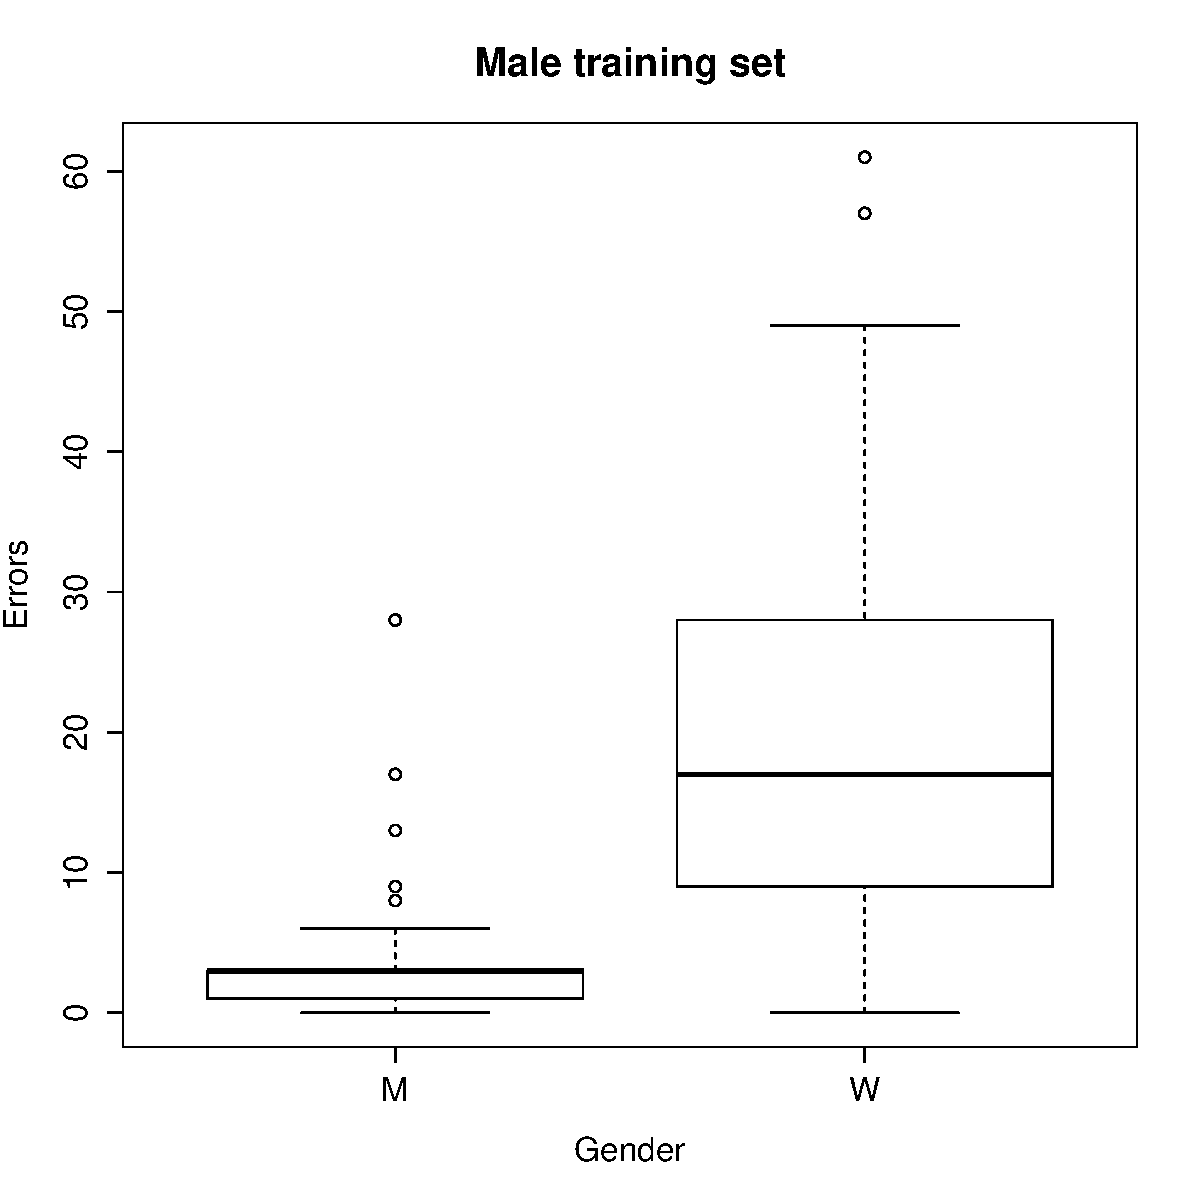
\includegraphics[width=\columnwidth]{male_only.pdf}
    \caption{\label{fig:male} Sentence error distributions of our system trained only on male speakers.}
  \end{subfigure}
\end{figure}
\begin{figure}[h]
  \ContinuedFloat%
  \begin{subfigure}{\columnwidth}
    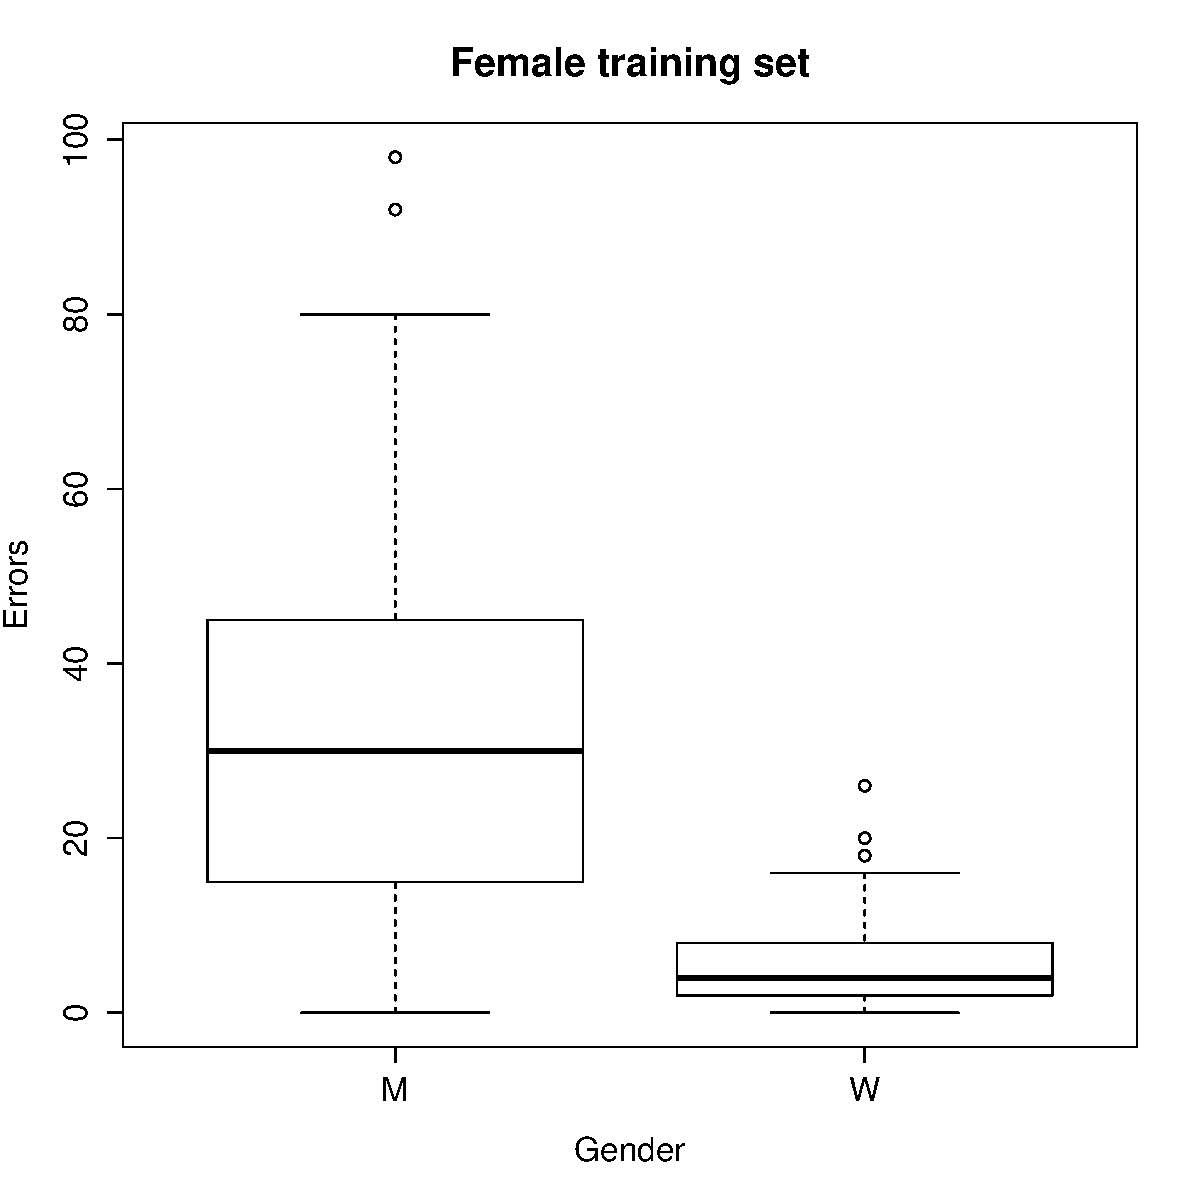
\includegraphics[width=\columnwidth]{female_only.pdf}
    \caption{\label{fig:female} Sentence error distributions of our system trained only on female speakers. }
  \end{subfigure}
  \begin{subfigure}{\columnwidth}
    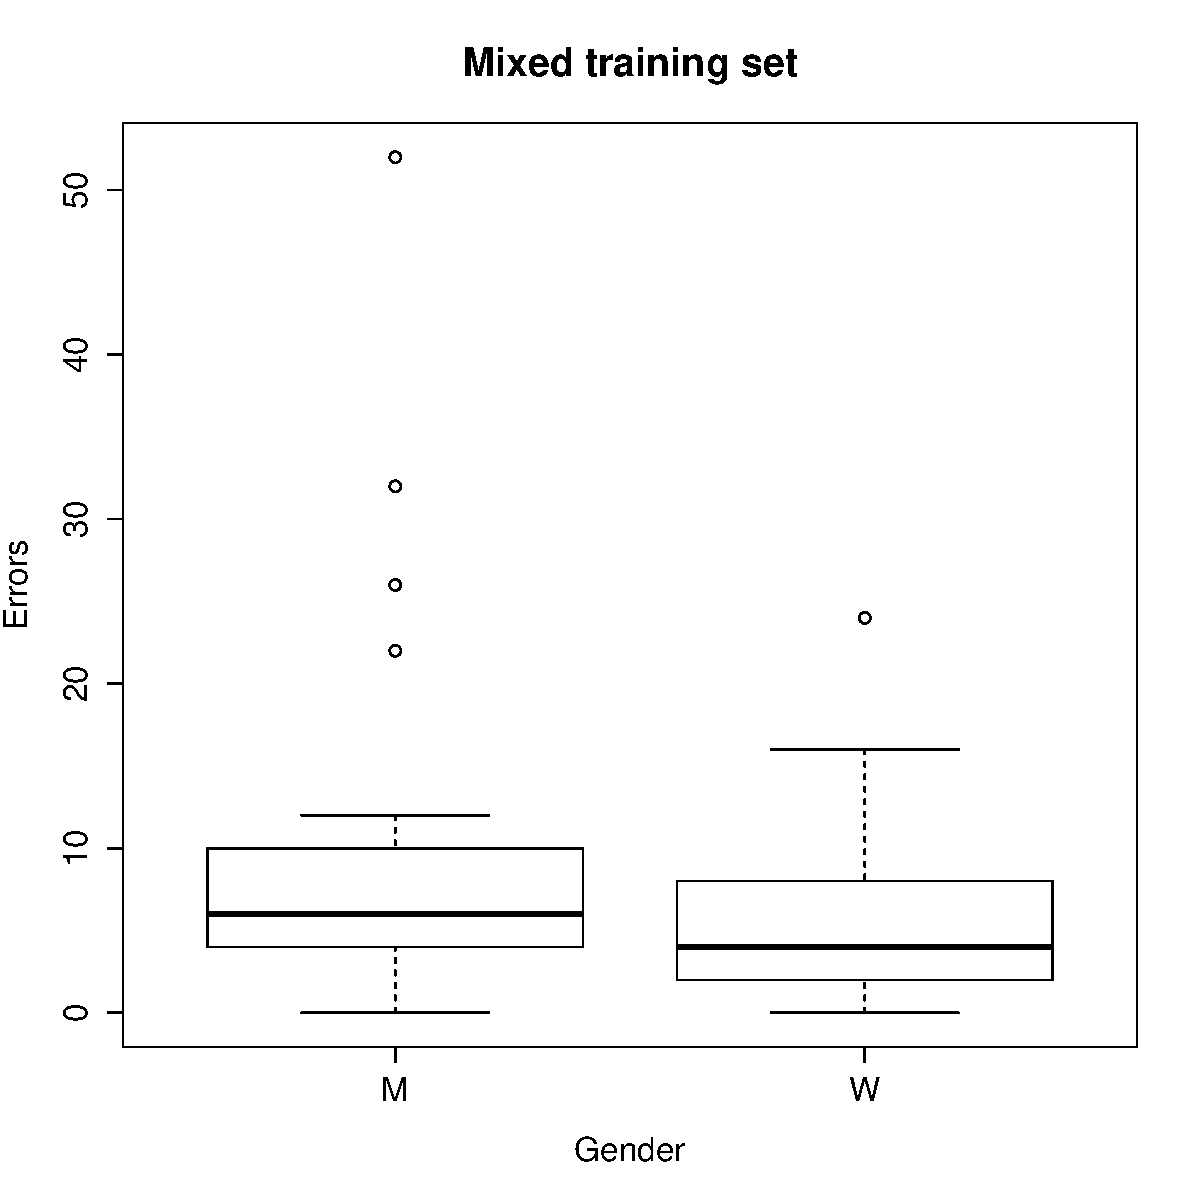
\includegraphics[width=\columnwidth]{mixed.pdf}
    \caption{\label{fig:mixed} Sentence error distributions of our system trained on speakers of both genders. }
  \end{subfigure}
  \caption{Sentence error distributions for different
  datasets.}\label{fig:boxplots}
\end{figure}

\end{document}
